\documentclass[a4paper]{scrartcl}
\setlength{\parindent}{0mm}


%\usepackage[utf8]{inputenc}
\usepackage[utf8]{inputenc}
\usepackage[ngerman]{babel}
\usepackage{amsmath}
\usepackage{fancyhdr}
\usepackage{dsfont}
\usepackage{lastpage}
\usepackage{paralist}
\usepackage{pifont}	%false \ding{55}  true \ding{52}
\usepackage{amssymb}
\usepackage{enumerate}
\usepackage{graphicx}

%Lightning
\usepackage{stmaryrd}

% \usepackage{amsthm} 
% \begin{proof}
% \end{proof}


\pagestyle{fancy}
\fancyhead[L]{Sommersemester 2016 \\ Maschinelles Lernen}
\fancyhead[C]{}
\fancyhead[R]{Nikolas Zeitler, Joshua Hartmann, Alexander Diegel}
\fancyfoot[L]{}
\fancyfoot[C]{\thepage /\pageref{LastPage}}
\fancyfoot[R]{}

\renewcommand{\textheight}{700px}
\renewcommand{\footskip}{10px}

\author{Nikolas Zeitler, Joshua Hartmann, Alexander Diegel}
\title{Übungsblatt 1}
\date{Abgabe bis: 23.04.15, 23:59 Uhr}



\begin{document}
\maketitle
\vspace{400px}
% DOCUMENT START
\newpage
\section{Aufgabe}
Beantworte bitte die folgenden Fragen in jeweils nicht mehr als drei Sätzen:
\begin{enumerate}[a)]
	\item \textbf{Was ist der Unterschied zwischen Regression und Klassifikation?}
	
	Klassifikation: teilt Ergebnisse in diskrete Gruppen ein.\\
	Regression: trifft kontinuierliche vorhersage für den Wert.
	
	\item \textbf{Angenommen man möchte anhand des Abstandes von Mittelfingerspitze und Ellbogen die Größe eines Menschen bestimmen. Bietet sich hier ein Klassifikations- oder Regressionsverfahren an?}
	
	Hier bietet sich eher ein Regressionsverfahren an, da die Körpergröße etwas kontinuierliches ist.
	
	\item \textbf{Angenommen man möchte analog das Geschlecht eines Menschen bestimmen. Bietet sich hier ein Klassifikationsoder Regressionsverfahren an?}
	
	Hier bietet sich ein Klassifikationsverfahren an, da das Geschlecht diskret in zwei Gruppen getrennt ist.
	
	\item \textbf{Was ist der Unterschied zwischen Supervised und Unsupervised Learning?}
	
	Beim Superviced Learning sind die Daten gelabeled, das heißt man gibt dem Algorithmus vor, was für ein Merkmal in dem Datensatz, mit dem er gerade trainiert wird, vorhanden ist.(Der Algorithmus bekommt Eingabe-Ausgabe-Wertepaare)\\
	Beim Unsuperviced Learning gibt man dem Algorithmus keinerlei vorgaben (er bekommt nur Eingabewerte), als Ergebnis kann er dann aber später auch nicht sagen, was genau er für Daten vor sich hat, aber er kann verschiedene Datensätze in bestimmten Clustern gruppieren, aus denen man dann selbst gewisse Schlüsse ziehen muss.
	
	\item \textbf{Wiederhole und nenne die grundlegenden Definitionen der Wahrscheinlichkeitsrechnung}
	
	\begin{enumerate}[(i)]
		\item Eine diskrete Zufallsvariable nimmt Werte aus einem diskreten Wertebereich an, eine kontinuierliche Zufallsvariable Werte aus einem kontinuierlichen Wertebereich.
		Ein Ereignis ist eine Menge von Ergebnissen eines Zufallsexperiments, dem eine Wahrscheinlichkeit zugeordnet werden kann. Bsp: Würfel-Ereignis “gerade Zahl würfeln” $\rightarrow$ Elementarereignisse \{2,4,6\} aus Ereignisraum \{1,2,3,4,5,6\}.
		
		\item Sie unterscheiden sich im Wertebereich, und P(X=i) ist im kontinuierlichen Fall immer 0, im diskreten Fall nicht.
		Die Wahrscheinlichkeitsdichtefunktion ist die Ableitung der Wahrscheinlichkeitsfunktion. 
		\item E(X) nimmt im kontinuierlichen ein X an, dass der “Mitte” der Wahrscheinlichkeitsdichtefunktion entspricht $\rightarrow$ welchen Wert nimmt die kontinuierliche Zufallsvariable im Mittel an.
		Im diskreten Fall kann das ein Wert sein, der zwischen zwei diskreten Werten liegt. Diesen Wert kann die Zufallsvariable dann nicht tatsächlich annehmen.\\
		ZB:. {0,1} $\rightarrow$ E(X) = 0.5, X ist aber entweder 0 oder 1.\\
		Definition: \\
		diskret: $E(X)=\sum_i(X_i*P(X_i))$ \\
		kontinuierlich: $E(X)= \int_{-\infty}^{\infty}(X*f)$ 
		
		\item 
		$VAR(X) = E[ X-E[X]^2]$\\
		$STDDEV(X) = \sqrt{VAR[X]}$\\
		VAR(X): Erwartete quadratische Abweichung der Zufallsvarbiablen von ihrem Mittelwert.\\
		STDDEV(X): Mittlerer Fehler der Zufallsvariablen\\
		VAR(X) lässt sich als E(Y) ausdrücken\\ $\rightarrow$ 
		$Y= (X-E[X])^2$
		
		\item $COV(X.Y) = E[(X-E[X)*(Y-E[Y))] = E[X*Y]-E[X]*E[Y]$\\
		Gibt wie stark zwei Zufallsvariablen gleichzeitig von ihrem Mittelwert abweichen.\\
		$>0$: X,Y sind positiv korreliert (Differenzen von X,Y zu ihrem Mittelwert haben gleiches Vorzeichen)\\
		$<0$: X,Y sind negativ korreliert (Differenzen von X,Y zu ihrem Mittelwert haben unterschiedliches Vorzeichen)\\
		$=0$: Dies ist dann der Fall wenn X,Y unabhängig sind es gilt aber lediglich X,Y unabhängig $\rightarrow$ $COV(X,Y)=0$ und NICHT $COV(X,Y)=0$ $\rightarrow$ X,Y unabhängig 
	\end{enumerate}
	
	\item \textbf{Liefert die Multiplikation zweier Wahrscheinlichkeitsdichten wieder eine solche? Begründung!}
	
	Nein, denn das Integral des Ergebnisses ist nicht 1 (siehe Beispiel in der Vorlesung). @Team was ist wenn normiert wird? Dann haben wir doch wieder eine??
\end{enumerate}

\section{Aufgabe}

\begin{enumerate}[a)]
	\item \textbf{Plotte die Standardnormalverteilung mit den oben genannten Parametern im Intervall [-8, 8].}
		
	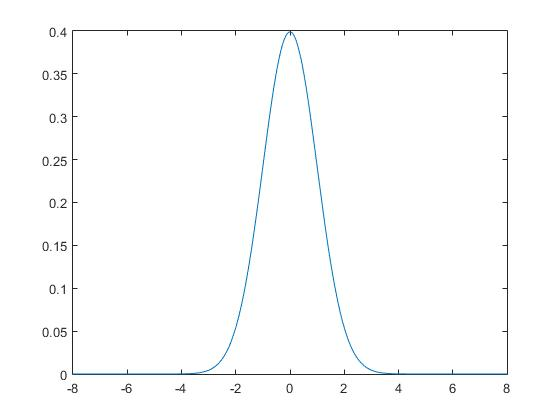
\includegraphics[width=.6\textwidth]{plots/2a_mu0_sigma1.jpg}
		
	
	\item \textbf{Verfahre wie in a), setze allerdings jeweils einmal $\mu = -2$ und $\sigma = 2$. Begründe die Änderung des Plots in zwei bis drei Sätzen.}
	
	$\mu = -2$:\\
	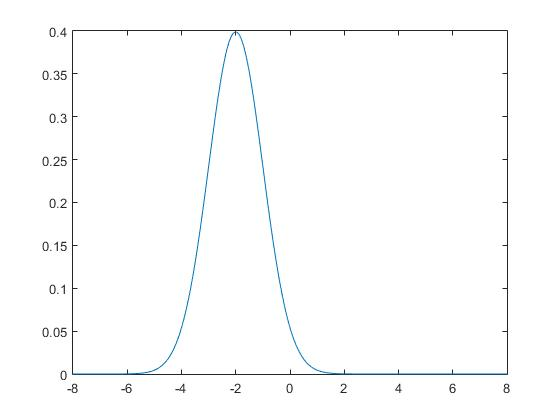
\includegraphics[width=.6\textwidth]{plots/2b_mu-2_sigma1.jpg}
	
	Der Plot wird nach links verschoben und das Maximum befindet sich bei $x=-2$, da der Erwartungswert $\mu = -2$ gesetzt wurde. 
	
	$\sigma = 2$:\\
	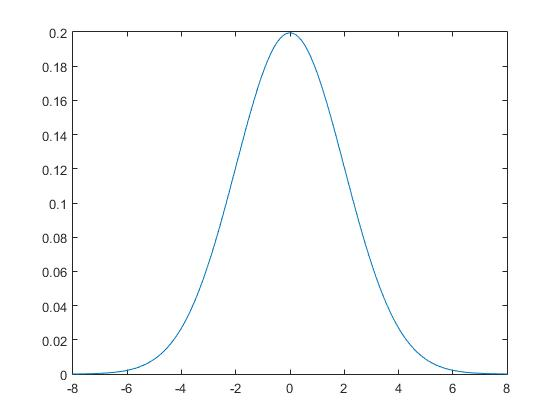
\includegraphics[width=.6\textwidth]{plots/2b_mu0_sigma2.jpg}
	
	Der Plot wird breiter, da die Standardabweichung vom Mittelwert größer ist. Der Plot wird auch flacher, da gleichzeitig das Integral weiterhin 1 sein muss.
	
	\item \textbf{Was bedeutet der Wert des Parameters $\mu = \mathbb{E}(X)$ für die Normalverteilung?}
	
	Er gibt das Maximum der Normalverteilung an.\\
	(Anmerkung Niki: Er gibt den Mittelwert der Normalverteilung an. Entpsrechend befindet an dieser Stelle der X-Wert des Hochpunktes)
	
	\item \textbf{Welche qualitative Bedeutung hat der Parameter $\sigma = \sqrt{Var(X)}$ für die Normalverteilung?}
	
	Er gibt an, wie weit Messwerte für gewöhnlich vom Mittelwert abweichen, also quasi die Breite der Glocke der Normalverteilung.
	
	\item \textbf{Wie bestimmt man mithilfe der Wahrscheinlichkeitsdichte f die Wahrscheinlichkeit des Ereignisses $\{ X \in [a,b]\}$, $\mathbb{P}(X\in[a,b]),a,b\in \mathbb{R}$ mit $a\le b$? }
	
	
	Man bildet das Integral $\mathbb{P}(X\in[a,b]) = \int_{a}^{b} f(x) dx$
	
	\item \textbf{Mit welcher Wahrscheinlichkeit nimmt X Werte an in den Intervallen}
	
	\begin{enumerate}[(i)]
		\item $I_1:$ 68,27\%
		\item $I_2:$ 95,45\%
		\item $I_3:$ 99,73\%
	\end{enumerate}	
	
	
	\item \textbf{Ist es für eine Wahrscheinlichkeitsdichte f möglich, dass ihr Wert f(x) an einer Stelle x ihres Definitionsbereiches größer als 1 ist? Begründe die Antwort!}
	
	An einer Stelle x ist das durchaus möglich, nur das Integral von f(x) muss gleich 1 sein. (Zum Beispiel zu sehen an einer Normalverteilung mit $\mu = 0$ und $\sigma = 0.1$)
	
\end{enumerate}

\section{Aufgabe}

\begin{enumerate}[a)]
	\item $\mu= (-1,1)$\\
	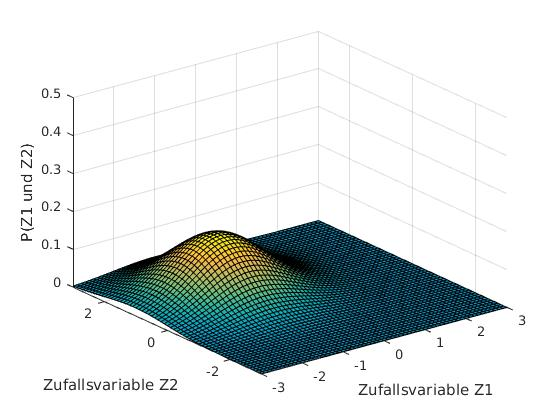
\includegraphics[width=.6\textwidth]{plots/3a_mu_1_1.jpg}\\
	Eine Änderung von $\mu=(0,0)$ nach $\mu=(-1,1)$ verschiebt den Erwartungswert der Zufallsvariable Z1 von 0 nach -1. Der Erwartungswert von Zufallsvariable Z2 wird von 0 nach 1 verschoben.\\
	Insgesamt befindet sich das neue Maxima der multivariate Normalverteilung bei $\mu=(-1,1)$.\\
	
	\item 
	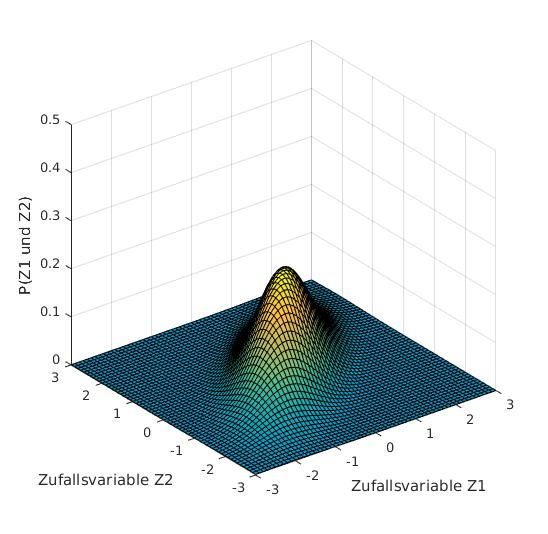
\includegraphics[width=.6\textwidth]{plots/3b_cov07.jpg}\\
	0.7: Beide Zufallsvariablen weichen gleichzeitig mit gleichem Vorzeichen von ihrem Mittelwert ab. Dadurch ergibt sich für die Abweichungen eine Ellipse (in der Grundfläche der Graphik), die auf der Geraden $y(x)=x$ verläuft.\\
	
	0.99: Ähnlich wie oben, allerdings korrelieren Z1 und Z2 nahezu maximal. Die Ellipsenform streckt sich entlang der Gerade $y(x)=x$.\\
	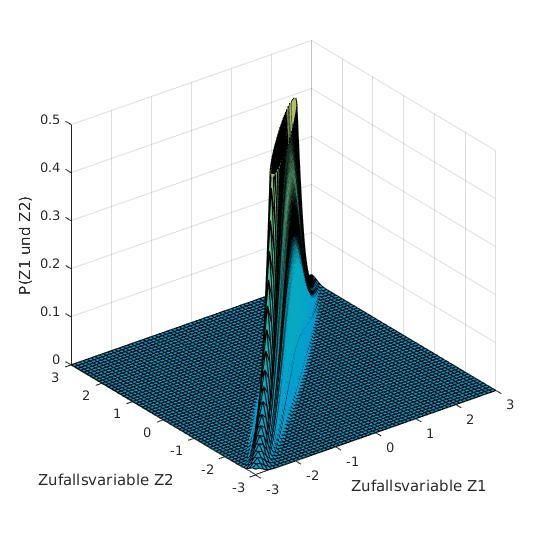
\includegraphics[width=.6\textwidth]{plots/3b_cov099.jpg}\\
	
	-0.7: Zufallsvariablen weichen gleichzeitig mit unterschiedlichem Vorzeichen von ihrem Mittelwert ab. Es ergibt sich eine Ellipse die auf der Geraden $y(x)=-x$ verläuft.\\	
	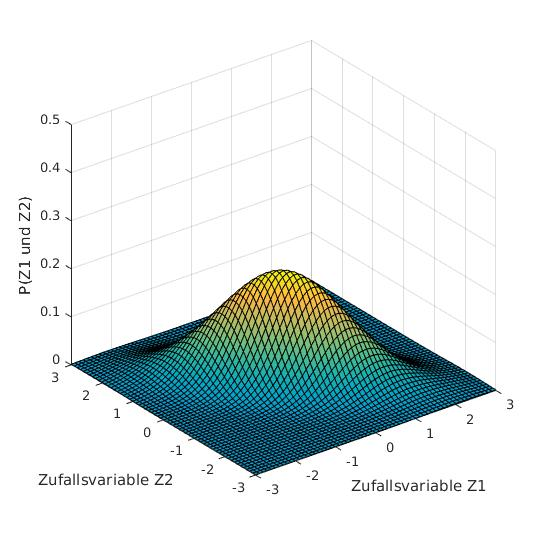
\includegraphics[width=.6\textwidth]{plots/3b_cov-07.jpg}\\

	-0.99: Nahezu maximal negative Korrelation.
	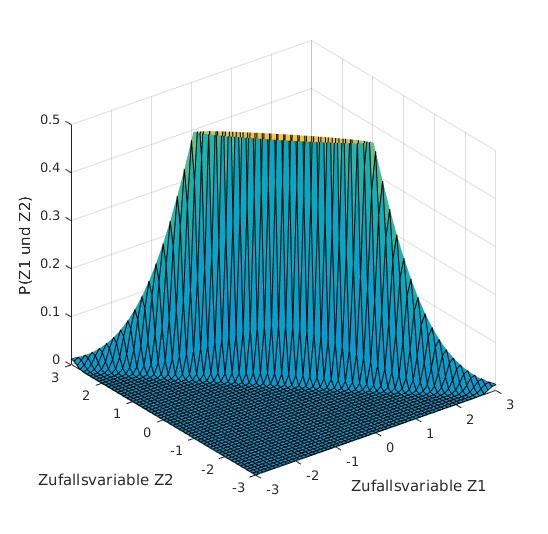
\includegraphics[width=.6\textwidth]{plots/3b_cov-099.jpg}\\
	
	\item 
	Korrelationskoeffizient sagt nichts über die Richtung des Zusammenhangs zweier Zufallsvariablen aus. Die Kovarianz dagegen schon.Der quadrierte Koeffizient gibt an, wie viel Prozent der Streuung einer Zufallsvariable durch die Streuung der anderen Zufallsvariablen erklärt werden können. Die Kovarianz betrachtet dagegen lediglich die gleichzeitige Abweichung der Zufallsvariablen von deren jeweiligen Mittelwert.\\
	
\end{enumerate}

\section{Aufgabe}

\begin{enumerate}[a)]
	\item 
	\item 
		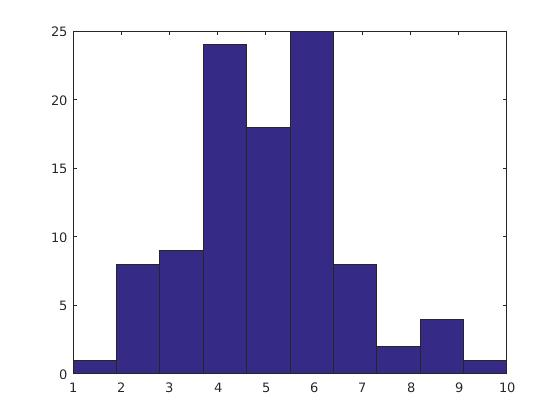
\includegraphics[width=.6\textwidth]{plots/4b.jpg}
	\item 
		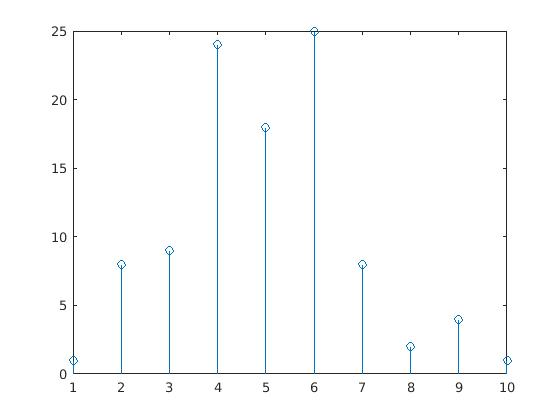
\includegraphics[width=.6\textwidth]{plots/4c.jpg}
	\item 
		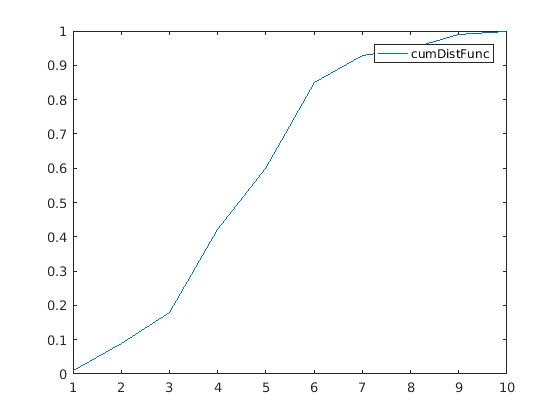
\includegraphics[width=.6\textwidth]{plots/4d.jpg}
	\item 
		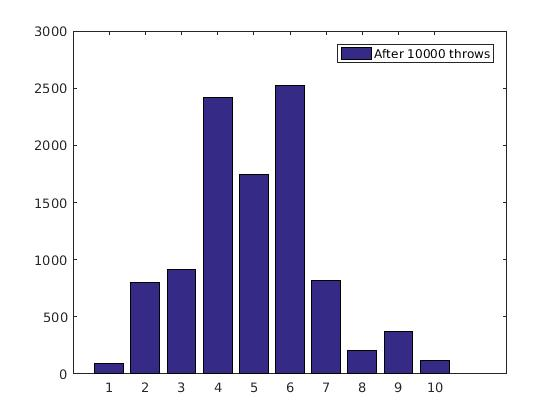
\includegraphics[width=.6\textwidth]{plots/4e.jpg}
	\item 
		Für bessere Ergebnisse sollte man den gezinkten Würfel öfters werfen. Hier wurde er nur 100-mal geworfen. Eine höhere Anzahl verbessert das Ergebnis.

	
\end{enumerate}

\end{document}